%!TEX root = Humanoids2013.tex
\section{Introduction}
\label{sec:introduction}

A crucial component that dramatically affects performance of robots is their actuation. Recent developments in this field have introduced fixed or physically adjustable compliant elements to enrich the dynamics of conventional motors. %\cite{SoftRoboticsDLR08, TsLaVaCa09}.%  (see SMART ACTUATORS and REVIEW VSA)
These devices provide advantages w.r.t.~rigid actuators, including higher peak performances, lower energy consumption and improved safety (see \cite{Pratt95,VanderborghtVHDLDB06,CGGBMTB11}, \cite{Taylor:2011}). This new tendency is the so called soft actuation, used for instance in manipulation \cite{SoftRoboticsDLR08}, or in humanoid design \cite{TsLaVaCa09}.

Among soft actuators, SEAs~\cite{Pratt95} have a linear compliant element between a high impedance actuator and the load. On the other hand, PEAs have an elastic element in parallel with the motor (i.e. between two links). Other examples of soft actuators are the Variable Stiffness Actuators (VSA), and the Variable Impedance Actuators (VIA). VSAs have an elastic transmission whose stiffness can be mechanically adjusted, while VIAs can include mechanisms (e.g.~brakes, dampers) allowing to change the output shaft impedance~\cite{CGGBDBTB12:2}.
% 
%  have a elastic element in series between the motor and the load. The latter allows also to change the motor's damping . 
Recent studies explore the role of such devices in performance enhancement, looking at very dynamic tasks. For instance, in \cite{AlbuSchaffer2011, Garabini2011} the objective is to optimally choose the stiffness to maximize the velocity of a VSA at a given final position with free final time. In \cite{CGGBDBTB12}, a new constraint is imposed, solving the same problem but with fixed terminal time.
% VSA VIJAYKUMAR %\cite{ViHo11}
% Optimal control is also addressed in \cite{nakanishi11} to achieve efficient actuators and control of a periodic motion for dynamical systems by exploiting intrinsic passive dynamics of VSA. %The methodology presented has not been applied to systems as walking or hopping robots. 
% One of the goals of humanoid robotics is to understand human dynamics as well as to reproduce it in simulation and hardware. However, SEA are non-commercial, and this means that most of them have been designed for specific applications \cite{Taylor:2011}, \cite{doi:10.1117/12.548000}. 
% Among the robots that use compliant actuation, \cite{4115608}, \cite{620132}, \cite{4115646}, \cite{MABEL}, \cite{4115607}, \cite{VanderborghtVHDLDB06}, \cite{ZVTCC2012}, for example in \cite{4115608} the compliance is tuned to have natural motion of the legs.
% In \cite{Hurst08} a monopod leg is presented with the knee joint actuated by a SEA. Experimental tests have shown that a suitable stiffness value reduces the mechanical work done by the motor during a stance phase while hopping in place.
% Motivations that pushed the development toward this direction arise in the intent of the robotics community to give humanoid robots the best characteristics of human beings. In fact, humans are low stiffness, low bandwidth systems (TODO cite), compared to most of the humanoid robots designed that have high bandwidth, and which are stiff \cite{Pratt95}, \cite{4115607}. 
 
\begin{figure}[t!]
\centering
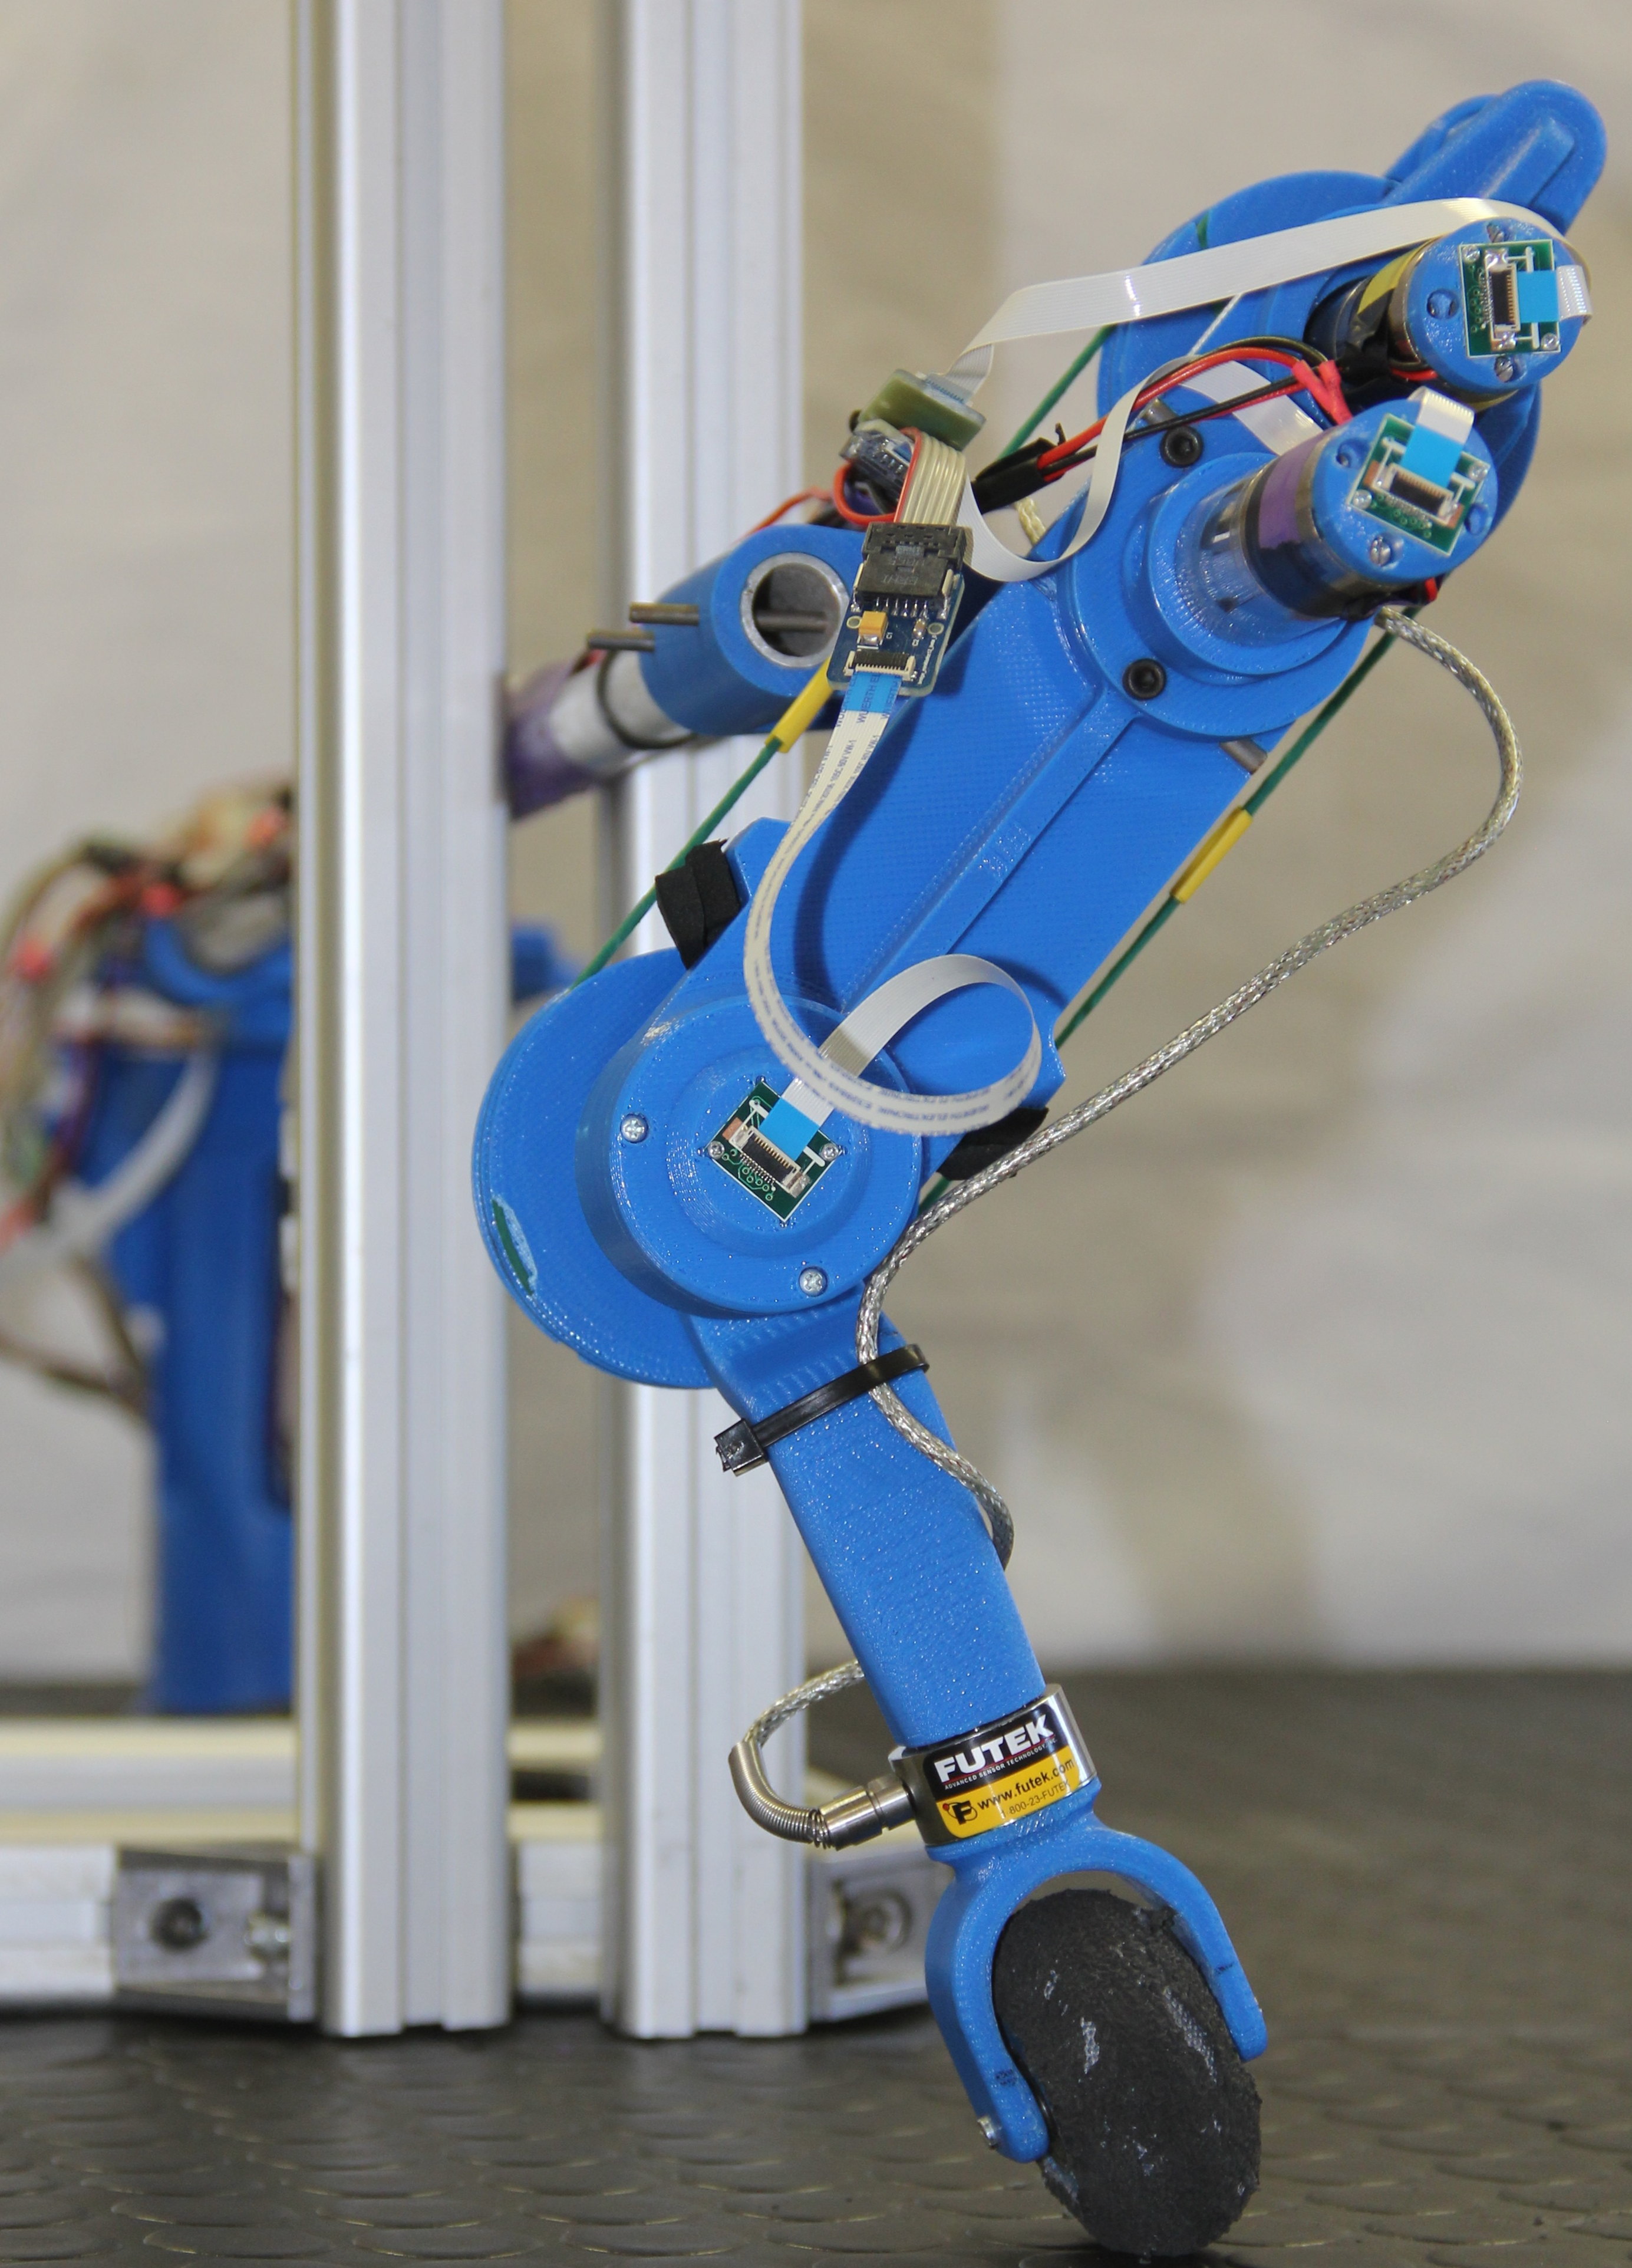
\includegraphics[width=0.7\columnwidth]{dwg/Saltarello}
\caption{The prototype of the Hopper used for experiments.}
\label{fig:Prototype}
\end{figure}
In this paper, we study the role of soft actuation in the reduction of the energy cost for mechanical systems that perform cyclic tasks. The objective is to determine, for given desired joint trajectories, the optimal stiffness value and spring pre-load such that a given cost functional is minimized.

% Fully actuated and underactuated dynamical systems using elastic actuation are considered. % Paragraph in which robots energy efficiency statistics 
% An analytical methodology to optimize the actuation parameters (joint stiffness and pre-load, the first in the SEA case or both in the PEA case), for given joint trajectories, is presented. 
% The method can be applied using different performance indices (based on squared torque, or squared mechanical power) to be chosen on the basis of the type of actuation. 
% Moreover, this work, holds up that the performance index depends on the desired joint trajectories as well as on the actuation parameters. 
% With the presented methodology, the general problem in which both joint trajectories and actuation parameters have to be simultaneously optimized, can be translated into a problem in which the optimization involves just the joint trajectories.
%In this work it is shown that he performance index also depends on the desired joint trajectories; therefore this methology is extended to find the optimal joint trajectories by solving a nonlinear optimization problem subject to constraints that depend on the dynamics and on the desired task.  
 % Finally, a planar model of a biped robot that includes the trunk is considered. %In this case, the optimal stiffness for each joint which minimizes its energy consumption for a given walking gait is found. 
% For measuring the performance we define the Cost of transport (CoT) as in \cite{MSTLDS2010}. This cost measures the specific mechanical energy spent by the actuators divided by the mass and the traveled distance. The mechanical energy is considered as the time integral of the absolute value of the power spent by the actuators. This definition assumes that the negative work of an actuator cannot be used and that no brake is present, so the negative work must be produced by the actuators. For the examples presented, the cycles have been selected to have a known behavior of the system. Applying the proposed method, the elastic constant for each joint are found.

In the literature, several papers try to solve the same problem addressed in this work. 
%%%%%%%%%%%%%%%%%%%%%%%%%%%%%%%%
%NIKOS ICRA '13
For instance, a systematic method to optimally tune the joint stiffness of multi Degrees of Freedom (DoFs) SEA robots based on resonance analysis and energy storage maximization criteria is presented in \cite{Nikos13}. A modal study was performed on the CoMAN (Compliant huMANoid) robot model, to derive the natural frequencies for different leg configurations during the single support walking phase. The joint stiffness was selected to set the resonances of the system, 
% by solving a constrained optimization problem with a cost function that 
maximizing the energy stored in the joint springs. 
% of the robot or the joint passive deflection for a given joint torque vector. 
% Moreover, authors consider to set joint stiffness for the walking robot, though 
However, in \cite{Nikos13}, the design of trajectories is not based on joint stiffness selection directly and an approach to find the optimal stiffness and pre-load for the PEA case has not been addressed yet. 
% In \cite{MSTLDS2010} the performance of a passive-dynamic swinging leg is shown through the evaluation of energy efficiency. The joint trajectories are not derived in the mentioned work, though the passive joint stiffness is used to reduce the energetic cost in the swing phase (in walking).
Walking gaits generation for biped robots has also been addressed as a nonlinear optimization problem in~\cite{Ott12}. The trajectories are obtained through cubic spline interpolation but joint compliance is not considered. In~\cite{Ting10}, an optimization is proposed to find feasible trajectories for a hopping robot. By constraining the problem, stable hopping of the rigid, underactuated robot is achieved.  

A control method for tracking cyclic trajectories is presented in~\cite{Kawamura09:2}, taking advantage of resonance of the dynamic systems and hence obtaining the optimal (constant, linear) stiffness value.  
In~\cite{Kawamura09:1} an energy saving control method was applied to a simulated biped walking model. The link trajectories for a 4 DoF PEA robot are obtained via minimization of a performance index based on the squared torque. However, as in~\cite{Kawamura09:2}, the SEA case is not considered. 

In this paper, we consider both fully actuated and underactuated dynamical systems using elastic actuation with either SEA or PEA providing an analytical methodology to optimize the actuation parameters for given joint trajectories. We show that the general problem in which both joint trajectories and actuation parameters have to be simultaneously optimized, can be translated into a problem in which the optimization would involve just the joint trajectories. However, in this paper the optimal characterization of the joint trajectories shape is not considered, showing only that, in case of sinusoidal trajectories the amplitude and the frequency play an important role in the reduction of the energy spent.

To show the effectiveness of the results we apply our method to a simple one-link robot manipulator tracking a sinusoidal joint trajectory and to a two-link robot manipulator performing a pick and place task. 
By several simulations, in both cases we show that the use of soft actuation allows to save energy w.r.t.~the stiff actuation case. For the pick and place task, optimized soft actuation allows to save up to 53\% of energy. 
% To show insights and application of the results of this paper we report three examples. First we briefly present the SEA one-DoF case study with a sinusoidal desired trajectory. For this problem the proposed method provides the stiffness that makes the natural frequency of the system equal to the frequency of the desired trajectory. 
% Then we present the case of two-DoF manipulator with SEA which performs a pick and place task. We will show that, in the best case, optimized soft actuation allows to save the XX\% of the total mechanical energy w.r.t. rigid actuation.
Finally, a prototype of a hopping robot with SEAs is presented (see Fig.~\ref{fig:Prototype}) and by experimentation we show that our method is applicable to existing systems whose model is unknown.
